\documentclass{article}

\usepackage{ctex}
\usepackage[top=0.7in,bottom=0.7in,left=0.5in,right=0.5in]{geometry}
\usepackage{array}
\usepackage{multirow}
\usepackage{graphicx}
\usepackage{subfigure}
\usepackage{fancyhdr}
\usepackage{lastpage}
\usepackage{extramarks}
\usepackage{amsmath}
\usepackage{listings}
\usepackage{fontspec}
\newfontfamily\consolas{Consolas}
\usepackage{xcolor} % 定制颜色
\definecolor{mygreen}{rgb}{0,0.6,0}
\definecolor{mygray}{rgb}{0.5,0.5,0.5}
\definecolor{mymauve}{rgb}{0.58,0,0.82}
\lstset{ %
backgroundcolor=\color{white},      % choose the background color
basicstyle=\footnotesize\ttfamily,  % size of fonts used for the code
columns=fullflexible,
tabsize=4,
breaklines=true,               % automatic line breaking only at whitespace
captionpos=b,                  % sets the caption-position to bottom
commentstyle=\color{mygreen},  % comment style
escapeinside={\%*}{*)},        % if you want to add LaTeX within your code
keywordstyle=\color{blue},     % keyword style
stringstyle=\color{mymauve}\ttfamily,  % string literal style
frame=single,
rulesepcolor=\color{red!20!green!20!blue!20},
% identifierstyle=\color{red},
language=c++,
}

\newcommand{\hmwkTitle}{哈夫曼编码压缩、解压文件\ 实验报告}
\newcommand{\hmwkClass}{数据结构}
\newcommand{\hmwkClassInstructor}{}
\newcommand{\hmwkAuthorName}{毛子恒\ 李臻\ 张梓靖}

\pagestyle{fancy}
\lhead{\hmwkAuthorName}
\chead{\hmwkClass\ : \hmwkTitle}
\rhead{\firstxmark}
\lfoot{\lastxmark}
\cfoot{\thepage}
\renewcommand\headrulewidth{0.4pt}
\renewcommand\footrulewidth{0.4pt}

\title{\hmwkClass\ :\hmwkTitle}
\author{\hmwkAuthorName}

\setcounter{tocdepth}{1}

\begin{document}

\maketitle

\section*{小组成员}

\setlength{\tabcolsep}{9mm}
{
    \begin{table}[htbp]
        \centering
        \begin{tabular}{llll}
            班级:2019211309 & 姓名:毛子恒 & 学号:2019211397 & 分工:代码\ 文档   \\

            班级:2019211310 & 姓名:李臻   & 学号:2019211458 & 分工:测试\ 文档   \\

            班级:2019211308 & 姓名:张梓靖 & 学号:2019211379 & 分工:可视化\ 文档 \\
        \end{tabular}
    \end{table}
}

\tableofcontents
\newpage

\section{需求分析}

\subsection{题目描述}

对于一个指定的文件,应用哈夫曼编码压缩文件,或者对本程序生成的压缩文件进行解压。

\subsection{输入描述}

程序从给定的二进制文件中读入数据。

\subsection{输出描述}

程序向给定的二进制文件中输出结果,向标准输出中输出提示。

压缩文件分为若干个部分,每个部分包含如下信息:

\begin{enumerate}
    \item 原字符串中包含的不同字符的个数;
    \item 哈夫曼树中每个节点存储的字符(非叶结点不存储字符)、结点左右孩子的序号;
    \item 原字符串的长度、压缩后位串的长度;
    \item 编码后的位串。
\end{enumerate}

输出分为五种情况:

\begin{enumerate}
    \item 输入合法,程序正常运行结束,此时结果存储在给定的二进制文件中,并在标准输出中打印提示信息。
    \item 输入不合法,程序向标准输出打印错误信息,并且要求重新输入或异常退出。
    \item 程序发生运行时错误,比如内存分配失败。此时程序没有输出。
\end{enumerate}

关于更多细节请参考5\ 用户使用说明部分。

\subsection{样例输入输出}

由于压缩后的二进制文件难以阅读,故通过转换程序(./bit2string.c)将该压缩文件转化成容易阅读的形式展现在本实验报告中,将不同数据以空格或换行符分隔,原本按每8位存储的位串转化成01字符串。

\subsubsection{样例输入输出1}

压缩。

【输入】

\begin{lstlisting}[
    basicstyle=\small\consolas]
aaababcd
\end{lstlisting}

【输出】

('\#'后的内容为注释)

\begin{lstlisting}[
    basicstyle=\small\consolas]
4     # 出现的不同字符的个数/哈夫曼树叶结点的个数
c     # 一个叶结点,其中存储字符c,没有左右孩子 
d
b
a
1 2   # 一个非叶结点,不存储字符,左右孩子分别是1、2
3 5
4 6
8 2   # 原串的长度,压缩后字符串的长度(2个字节)
0001001011011100 # 压缩后的位串
\end{lstlisting}

\subsubsection{样例输入输出2}

压缩。

【输入】

\begin{lstlisting}[
    basicstyle=\small\consolas]
!#$""$#$"$$"!!"!$$#"$#"$"$!$#$!"!$!#"#!""#"!!!#"##"!$$$"#"$"$"$#!$$"$#!"#$##!!"#"#!!##!#$"!""$!"!#$$
\end{lstlisting}

【输出】

\begin{lstlisting}[
    basicstyle=\small\consolas]
4
#
!
"
$
1 2
3 4
5 6
100 25
010011101011001110111110010110011111001011001011101101110011011001110100100001101000100101010010000010011111111000
10111011101100011111101100011000110000010110001000010100000100111001101011011001001111
\end{lstlisting}

\subsubsection{样例输入输出3}

压缩。

【输入】

\begin{lstlisting}[
    basicstyle=\small\consolas]
1>8#2$'&'-).1%2/1:)/,8;2!3>(/69",#&7;>#$</%'=-=>+2#5&>!)5;(<96&;>0,7,;:/.)7$$/%5-(67933<(';==4464!12
\end{lstlisting}

【输出】

\begin{lstlisting}[
    basicstyle=\small\consolas]
29
"
+
0
.
:
8
-
5
9
<
!
4
3
%
)
'
&
$
#
=
7
6
1
,
(
2
>
;
/
1 2
3 30
4 5
6 31
7 8
9 10
11 12
13 14
15 32
16 17
18 19
20 21
22 23
24 25
26 33
27 34
28 35
29 36
37 38
39 40
41 42
43 44
45 46
47 48
49 50
51 52
53 54
55 56
100 60
111110100001101101100101101011000110011100001010101101011101111110101001010001111110111110110100000000011001100010
100101010001000001100011110011100011110000011011110011110101100100110111101001111100010101110001110001010111000100
001111100101101101011110010100100101011001011011000010111101110111101100101100100001110000011101000001101011111000
101110101101110111010110101000101010101101010000111110111010111010100101000111100011100001101110011100100111001111
110100111001011111001000
\end{lstlisting}

\subsubsection{样例输入输出4}

解压。

【输入】

\begin{lstlisting}[
    basicstyle=\small\consolas]
4
c
d
b
a
1 2
3 5
4 6
8 2
0001001011011100
\end{lstlisting}

【输出】

\begin{lstlisting}[
    basicstyle=\small\consolas]
aaababcd
\end{lstlisting}

\subsubsection{样例输入输出5}

解压。

【输入】

\begin{lstlisting}[
    basicstyle=\small\consolas]
4
#
!
"
$
1 2
3 4
5 6
100 25
010011101011001110111110010110011111001011001011101101110011011001110100100001101000100101010010000010011111111000
10111011101100011111101100011000110000010110001000010100000100111001101011011001001111
\end{lstlisting}

【输出】

\begin{lstlisting}[
    basicstyle=\small\consolas]
!#$""$#$"$$"!!"!$$#"$#"$"$!$#$!"!$!#"#!""#"!!!#"##"!$$$"#"$"$"$#!$$"$#!"#$##!!"#"#!!##!#$"!""$!"!#$$
\end{lstlisting}

\subsection{程序功能}

对于压缩过程,程序构造哈夫曼树并且对文件进行压缩,将需要的解码信息和压缩后的位串保存到压缩文件中。

对于解压过程,程序从压缩文件中读入解码信息和位串,并利用哈夫曼树进行解压。

\section{概要设计}

\subsection{问题解决的思路}

构造哈夫曼树进行压缩、解压过程。

\subsection{哈夫曼编码的设计}

\begin{lstlisting}[language={C},
    numbers=left,
    numberstyle=\tiny\consolas,
    basicstyle=\small\consolas]
\end{lstlisting}

\subsection{主程序的流程}

\begin{enumerate}
    \item 获取输入,判断是否合法
    \item 如果合法,则调用压缩/解压函数
\end{enumerate}

\subsection{各程序模块之间的层次关系}

程序模块层次关系图如图1。

\begin{figure}[htbp]

    % \centering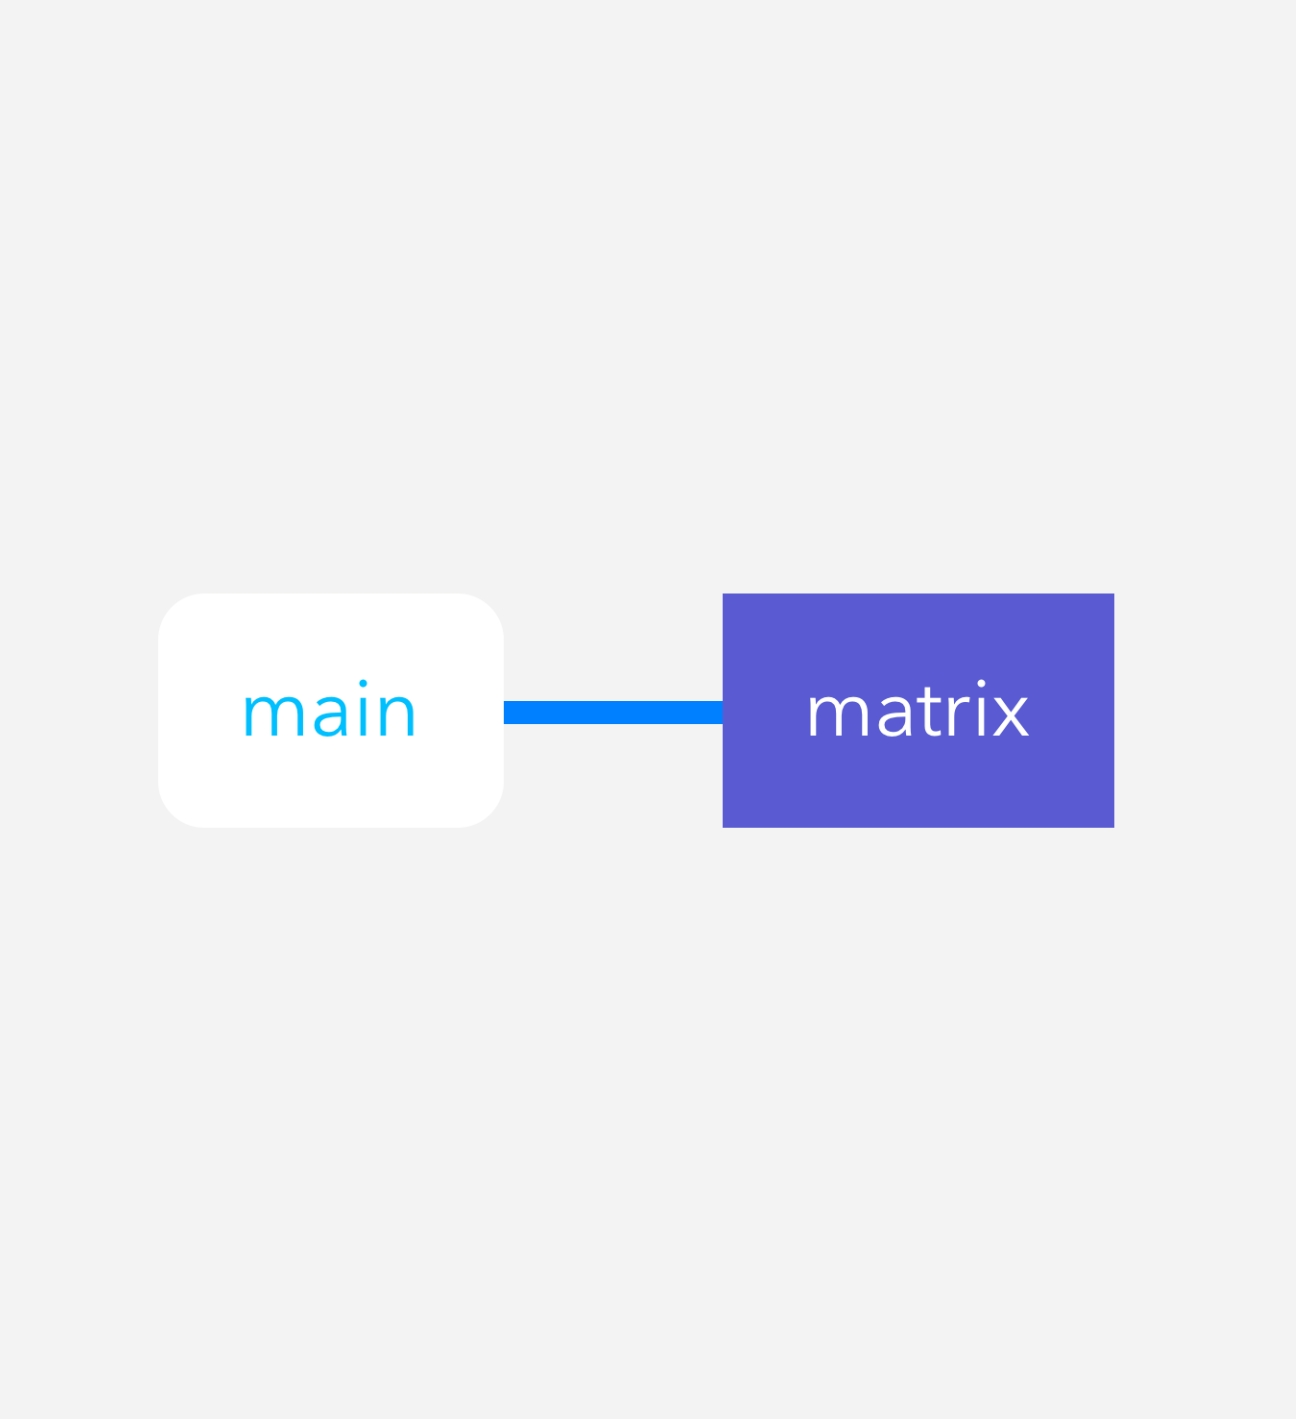
\includegraphics[width=0.4\textwidth]{./Images/pic3_1.png}

    \caption{程序模块层次关系}

\end{figure}

\section{详细设计}

\subsection{哈夫曼编码的实现}

哈夫曼编码的设计中基本操作的伪代码算法如下:

\begin{lstlisting}[language={C},
    numbers=left,
    numberstyle=\tiny\consolas,
    basicstyle=\small\consolas]
\end{lstlisting}

\subsection{函数的调用关系图}

函数调用关系图如图2。

\begin{figure}[htbp]

    % \centering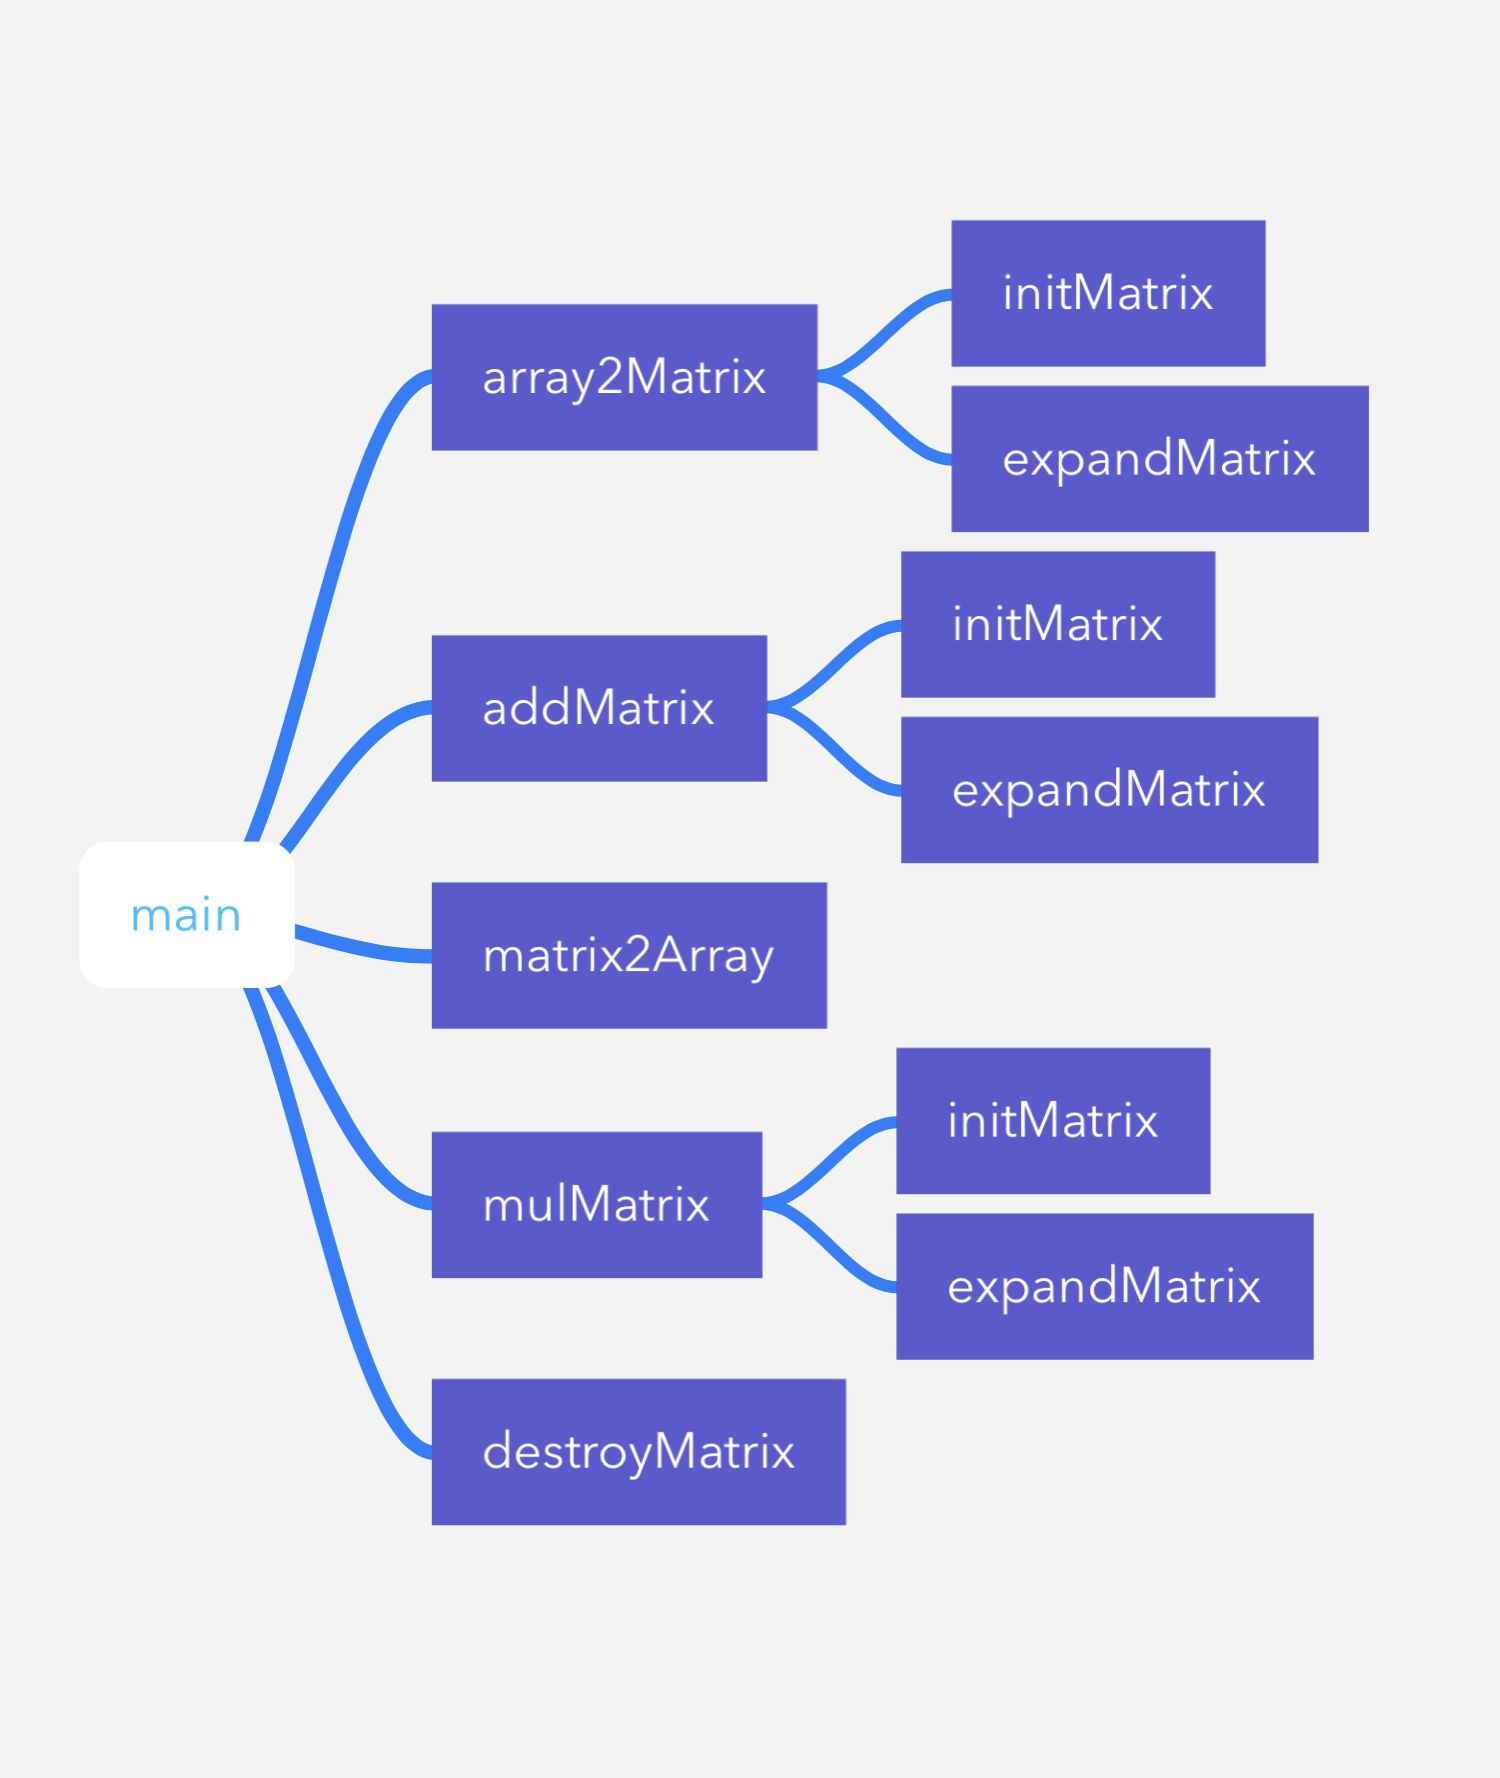
\includegraphics[width=0.4\textwidth]{./Images/pic3_2.png}

    \caption{函数调用关系图}

\end{figure}

\section{调试分析报告}

\subsection{调试过程中遇到的问题和思考}

程序在一些小细节中出现了问题,比如$val$数组需要多分配一个空间,矩阵相乘后$c$矩阵的列数等于$b$矩阵的列数。

初次实现矩阵相加算法时设计有误,使得两个矩阵的某个对应位置只要有一个为零,就会忽略这个位置,这个问题通过if判断修复。

在随机测试中发现数据规模较大时结果很容易超出int类型的范围,故矩阵元素采用long long类型。

\subsection{设计实现的回顾讨论}

由于二维数组的内存分配、函数传参较为复杂,所以输入、输出时使用一维数组存储的矩阵。

期望矩阵的规模不超过$10^3$,所以$MATRIXINCREASESIZE$常量的值设置为$10^5$。

\subsection{算法复杂度分析}

initMatrix, expandMatrix, destroyMatrix函数的复杂度为$O(1)$

array2Matrix, matrix2Array, addMatrix函数的复杂度为$O(n^2)$,mulMatrix函数的复杂度为$O(n^3)$,视矩阵的稀疏程度,算法的时间复杂度会有常数级别的优化。在本报告的最后部分有讨论。

主函数的时间复杂度为$O(n^2)$,整体时间复杂度为$O(n^3)$。

整体空间复杂度为$O(n^2)$。

\subsection{改进设想的经验和体会}

\subsubsection{改进1}

可以在输入/输出时简化数组存储的矩阵和三元组表存储的矩阵之间转化的过程,会有常数级别的优化。

\section{用户使用说明}

使用gcc编译生成可执行文件。

\begin{lstlisting}[language={bash},
    basicstyle=\small\consolas]
gcc -o main -std=c11 main.c matrix.c
\end{lstlisting}

执行可执行文件:

\begin{lstlisting}[language={bash},
    basicstyle=\small\consolas]
./main
\end{lstlisting}

在Windows cmd下:

\begin{lstlisting}[language={bash},
    basicstyle=\small\consolas]
main
\end{lstlisting}

之后通过标准输入输入数据,输入格式参考1.2节的输入描述,结果通过标准输出返回。如果输入合法并且程序正常运行结束,主函数返回值为0。

\section{测试结果}

测试环节分为三个步骤。

\subsection{测试第一部分}

对1.4节给出的样例进行测试。

\subsection{测试第二部分}

测试边界条件。

【输入】

\begin{lstlisting}[
    basicstyle=\small\consolas]
1 0
1 1
2
\end{lstlisting}

【输出】

\begin{lstlisting}[
    basicstyle=\small\consolas]
Please check your input.
\end{lstlisting}

【输入】

\begin{lstlisting}[
    basicstyle=\small\consolas]
4 3
7 0 6
0 0 5
1 0 0
0 0 2
3 3
5 7 0
0 3 0
1 3 5
\end{lstlisting}

【输出】

\begin{lstlisting}[
    basicstyle=\small\consolas]
Cannot add matrix A and B, An != Bn.
41 67 30 
5 15 25 
5 7 0 
2 6 10 
\end{lstlisting}

【输入】

\begin{lstlisting}[
    basicstyle=\small\consolas]
3 3
7 0 6
1 0 4
1 0 0
3 4
5 7 0 1
0 3 0 0
1 3 5 0
\end{lstlisting}

【输出】

\begin{lstlisting}[
    basicstyle=\small\consolas]
Cannot add matrix A and B, Am != Bm.
41 67 30 7 
9 19 20 1 
5 7 0 1 
\end{lstlisting}

【输入】

\begin{lstlisting}[
    basicstyle=\small\consolas]
3 4
7 0 6 4
1 0 4 0
1 0 0 6
3 4
5 7 0 1
0 3 0 0
1 3 5 0
\end{lstlisting}

【输出】

\begin{lstlisting}[
    basicstyle=\small\consolas]
12 7 6 5 
1 3 4 0 
2 3 5 6 
Cannot multiply matrix A and B, Am != Bn.
\end{lstlisting}

\subsection{测试第三部分}

将原解法与二维数组实现的矩阵加法和乘法(testing/test.c)比对。

测试在macOS\ Catalina\ 10.15.6下进行。

在$n<=10$,$n<=100$,$n<=1000$的范围下分别随机生成1000组测试数据,分别传入main和test,并且比对两程序的输出。

3000组数据中两程序的输出均相同。

数据生成程序(testing/data.cpp)如下:

\begin{lstlisting}[language={C++},
    numbers=left,
    numberstyle=\tiny\consolas,
    basicstyle=\small\consolas]
#include <bits/stdc++.h>
using namespace std;

const int SIZE = 1e3, PERCENT = 50;

int main()
{
    srand(time(0));
    int n = rand() % SIZE + 1;
    printf("%d %d\n", n, n);
    for (int i = 1; i <= n; ++i)
    {
        for (int j = 1; j <= n; ++j)
            printf("%d ", rand() % 100 > PERCENT ? 0 : rand() % 1000 + 1);
        puts("");
    }
    printf("%d %d\n", n, n);
    for (int i = 1; i <= n; ++i)
    {
        for (int j = 1; j <= n; ++j)
            printf("%d ", rand() % 100 > PERCENT ? 0 : rand() % 1000 + 1);
        puts("");
    }
    return 0;
}
\end{lstlisting}

比对脚本(testing/chk.sh)如下:

\begin{lstlisting}[language={bash},
    numbers=left,
    numberstyle=\tiny\consolas,
    basicstyle=\small\consolas]
for i in {1..1000}
do
    sleep 1
    ./data >in.in
    ./main <in.in >out.out
    ./test <in.in >out1.out
    if ! diff out.out out1.out
    then
        break
    fi
    echo "Correct"
done
\end{lstlisting}

\section{可视化}

随机生成若干组数据,由三元组表实现和二维数组实现分别计算,比对运行时间,并且使用JavaScript将结果可视化。

比对脚本(testing/timecount.py)如下:

\begin{lstlisting}[language={python},
    numbers=left,
    numberstyle=\tiny\consolas,
    basicstyle=\small\consolas]
import os
import json
import time
a = []
b = []
for i in range(100):
    os.system("./data >in.in")
    starttime = time.time()
    os.system("./main <in.in >out.out")
    endtime = time.time()
    a.append(endtime-starttime)
    starttime = time.time()
    os.system("./test <in.in >out1.out")
    endtime = time.time()
    b.append(endtime-starttime)
    print(i)

json_str = json.dumps([a, b])
with open("80%result.json", mode="w") as file:
    file.write(json_str)
\end{lstlisting}

数据规模如下:

$n=1000$,$20\%$的元素是0、$50\%$的元素是0、$80\%$的元素是0的数据各100组,共300组数据。

\subsubsection{实现细节}

利用已有的时间数据,使用Highcharts库绘制二维柱状图,比较两种算法的运行时间差距。

\subsubsection{用户使用说明}

使用现代浏览器打开Chart/index.html,即可看到柱状图,将鼠标指针放到某个柱上可以看到对应的值。

\subsubsection{示例}

见图3。

\begin{figure}[htbp]
    
    % \centering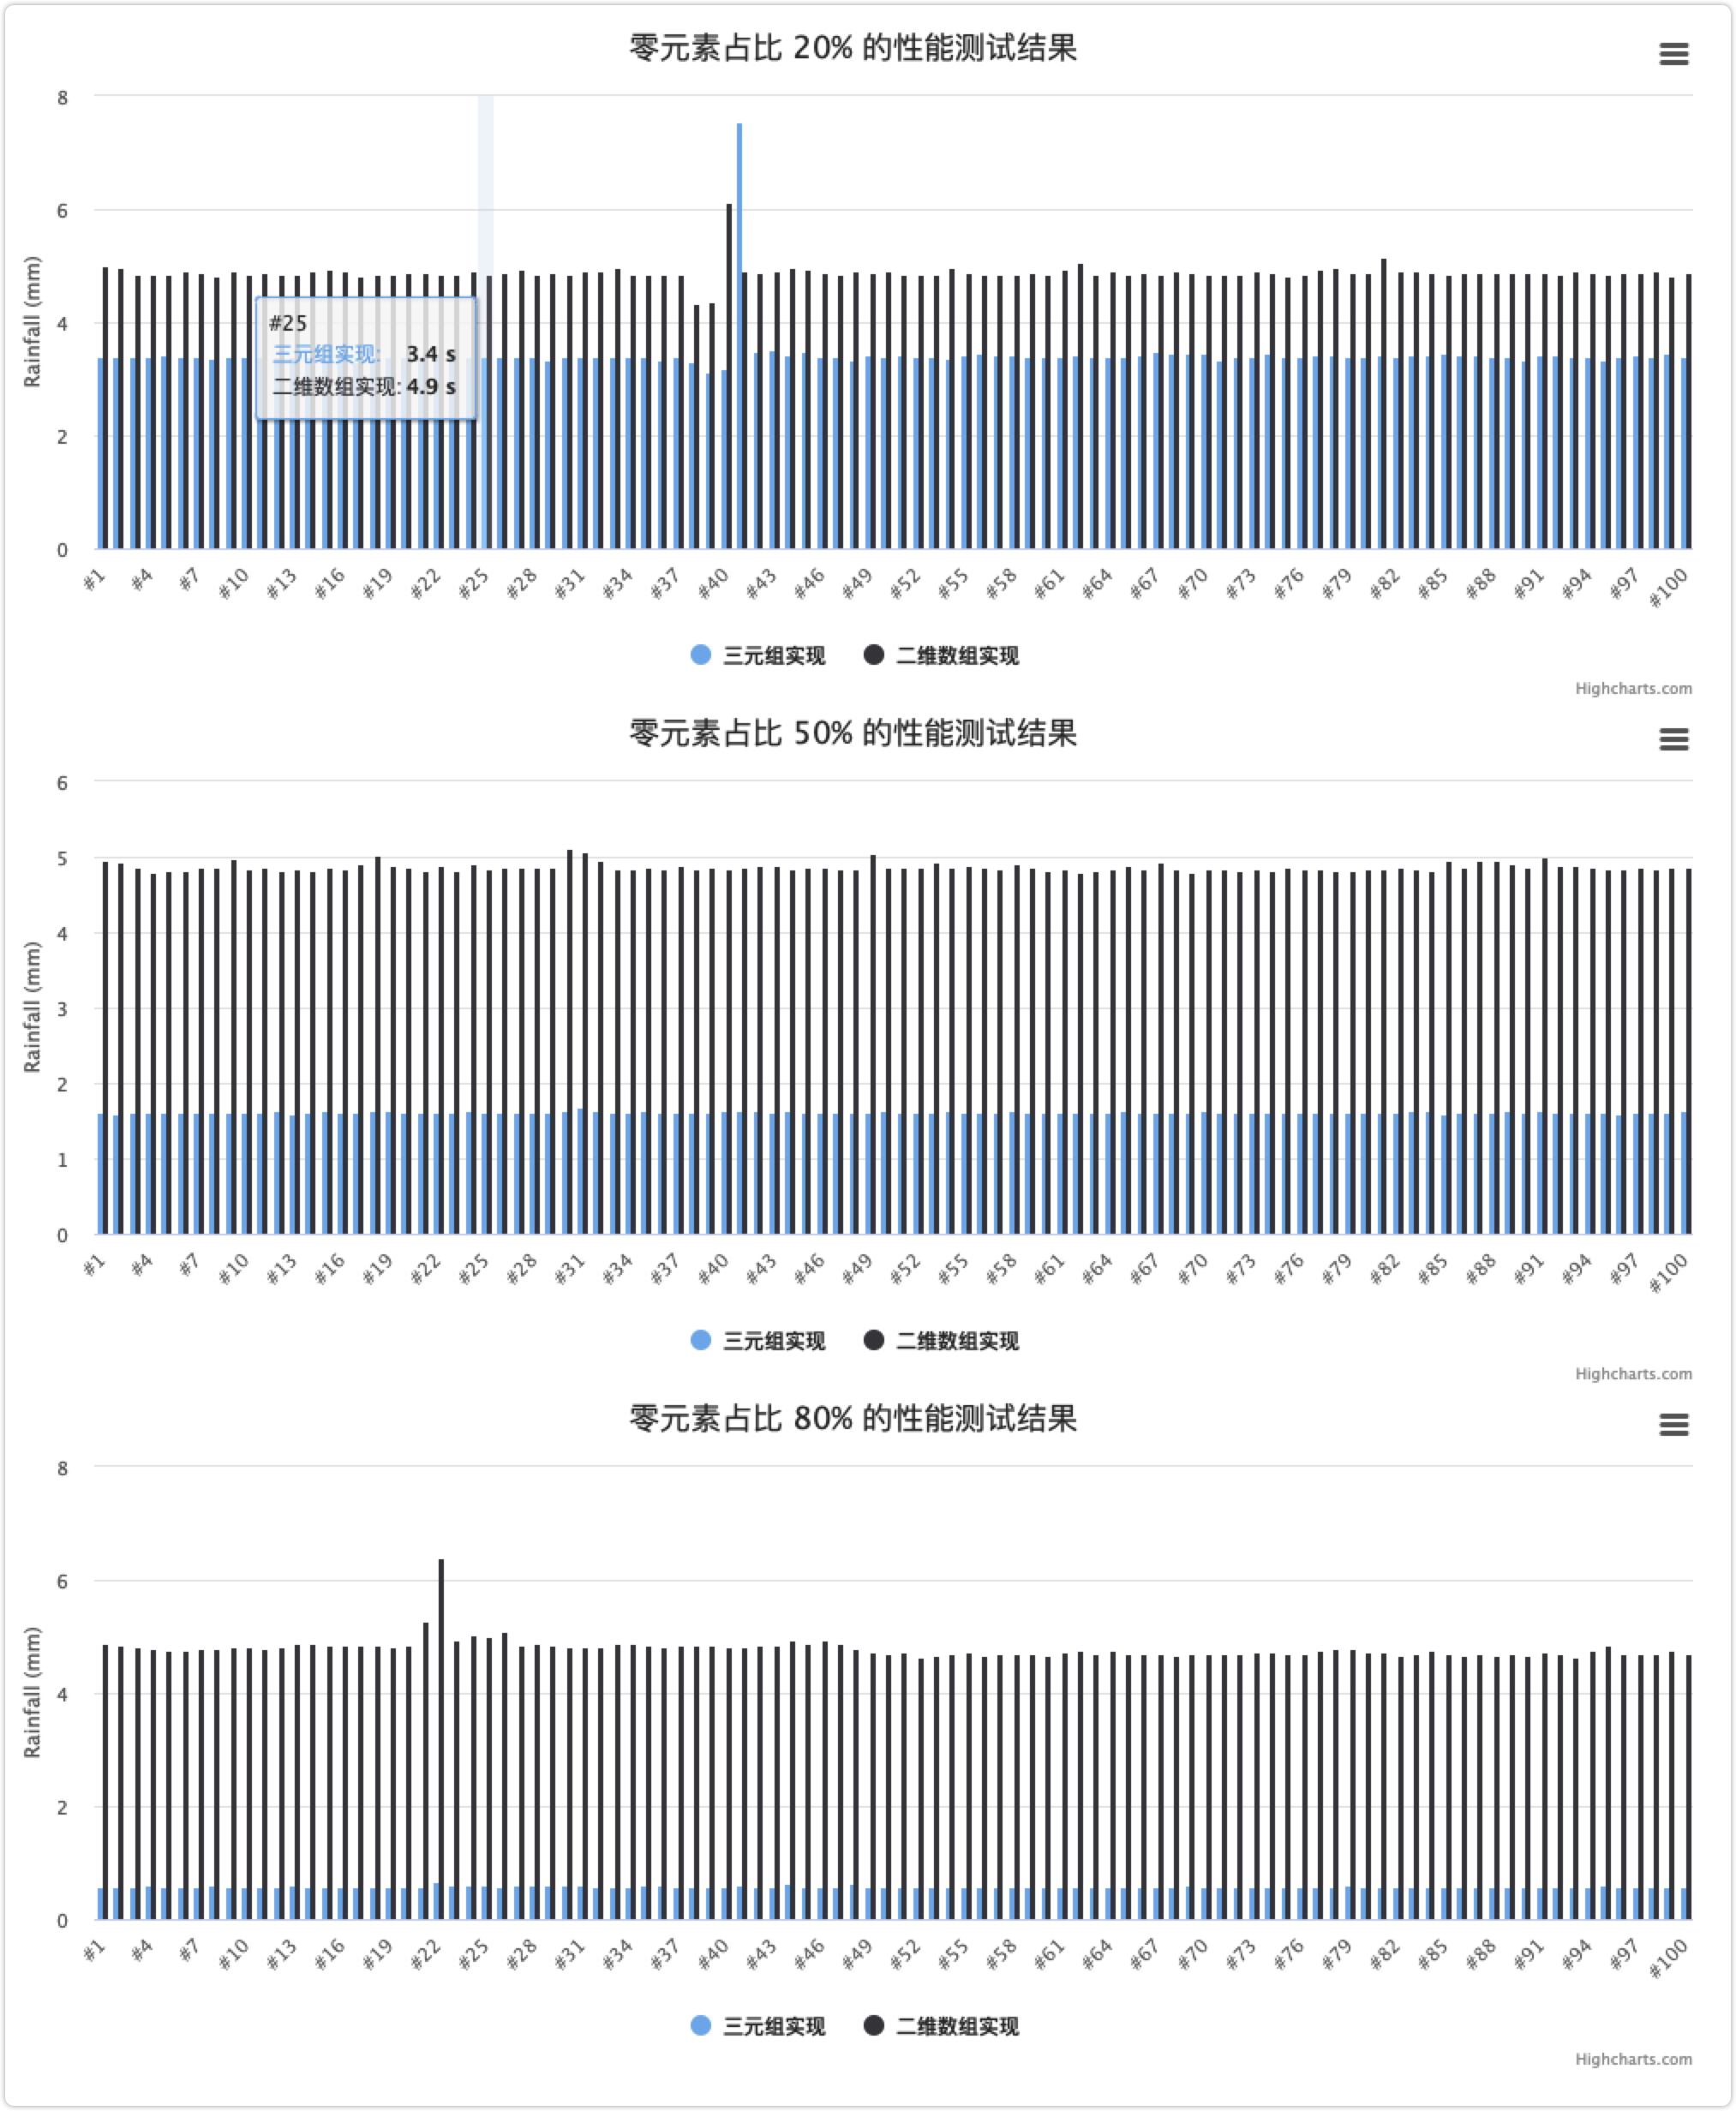
\includegraphics[width=0.9\textwidth]{./Images/pic3_3.png}
    
    \caption{可视化示例}
    
\end{figure}

\subsubsection{结论}

可以看出在规模较大的数据中,相比二维数组的实现,三元组表的实现在绝大多数情况下都有明显的性能优势,并且当矩阵越稀疏时性能优势越明显。

\end{document}
